\documentclass[twoside]{book}

% Packages required by doxygen
\usepackage{fixltx2e}
\usepackage{calc}
\usepackage{doxygen}
\usepackage[export]{adjustbox} % also loads graphicx
\usepackage{graphicx}
\usepackage[utf8]{inputenc}
\usepackage{makeidx}
\usepackage{multicol}
\usepackage{multirow}
\PassOptionsToPackage{warn}{textcomp}
\usepackage{textcomp}
\usepackage[nointegrals]{wasysym}
\usepackage[table]{xcolor}

% Font selection
\usepackage[T1]{fontenc}
\usepackage[scaled=.90]{helvet}
\usepackage{courier}
\usepackage{amssymb}
\usepackage{sectsty}
\renewcommand{\familydefault}{\sfdefault}
\allsectionsfont{%
  \fontseries{bc}\selectfont%
  \color{darkgray}%
}
\renewcommand{\DoxyLabelFont}{%
  \fontseries{bc}\selectfont%
  \color{darkgray}%
}
\newcommand{\+}{\discretionary{\mbox{\scriptsize$\hookleftarrow$}}{}{}}

% Page & text layout
\usepackage{geometry}
\geometry{%
  a4paper,%
  top=2.5cm,%
  bottom=2.5cm,%
  left=2.5cm,%
  right=2.5cm%
}
\tolerance=750
\hfuzz=15pt
\hbadness=750
\setlength{\emergencystretch}{15pt}
\setlength{\parindent}{0cm}
\setlength{\parskip}{3ex plus 2ex minus 2ex}
\makeatletter
\renewcommand{\paragraph}{%
  \@startsection{paragraph}{4}{0ex}{-1.0ex}{1.0ex}{%
    \normalfont\normalsize\bfseries\SS@parafont%
  }%
}
\renewcommand{\subparagraph}{%
  \@startsection{subparagraph}{5}{0ex}{-1.0ex}{1.0ex}{%
    \normalfont\normalsize\bfseries\SS@subparafont%
  }%
}
\makeatother

% Headers & footers
\usepackage{fancyhdr}
\pagestyle{fancyplain}
\fancyhead[LE]{\fancyplain{}{\bfseries\thepage}}
\fancyhead[CE]{\fancyplain{}{}}
\fancyhead[RE]{\fancyplain{}{\bfseries\leftmark}}
\fancyhead[LO]{\fancyplain{}{\bfseries\rightmark}}
\fancyhead[CO]{\fancyplain{}{}}
\fancyhead[RO]{\fancyplain{}{\bfseries\thepage}}
\fancyfoot[LE]{\fancyplain{}{}}
\fancyfoot[CE]{\fancyplain{}{}}
\fancyfoot[RE]{\fancyplain{}{\bfseries\scriptsize Generated by Doxygen }}
\fancyfoot[LO]{\fancyplain{}{\bfseries\scriptsize Generated by Doxygen }}
\fancyfoot[CO]{\fancyplain{}{}}
\fancyfoot[RO]{\fancyplain{}{}}
\renewcommand{\footrulewidth}{0.4pt}
\renewcommand{\chaptermark}[1]{%
  \markboth{#1}{}%
}
\renewcommand{\sectionmark}[1]{%
  \markright{\thesection\ #1}%
}

% Indices & bibliography
\usepackage{natbib}
\usepackage[titles]{tocloft}
\setcounter{tocdepth}{3}
\setcounter{secnumdepth}{5}
\makeindex

% Hyperlinks (required, but should be loaded last)
\usepackage{ifpdf}
\ifpdf
  \usepackage[pdftex,pagebackref=true]{hyperref}
\else
  \usepackage[ps2pdf,pagebackref=true]{hyperref}
\fi
\hypersetup{%
  colorlinks=true,%
  linkcolor=blue,%
  citecolor=blue,%
  unicode%
}

% Custom commands
\newcommand{\clearemptydoublepage}{%
  \newpage{\pagestyle{empty}\cleardoublepage}%
}

\usepackage{caption}
\captionsetup{labelsep=space,justification=centering,font={bf},singlelinecheck=off,skip=4pt,position=top}

%===== C O N T E N T S =====

\begin{document}

% Titlepage & ToC
\hypersetup{pageanchor=false,
             bookmarksnumbered=true,
             pdfencoding=unicode
            }
\pagenumbering{alph}
\begin{titlepage}
\vspace*{7cm}
\begin{center}%
{\Large My Project }\\
\vspace*{1cm}
{\large Generated by Doxygen 1.8.12}\\
\end{center}
\end{titlepage}
\clearemptydoublepage
\pagenumbering{roman}
\tableofcontents
\clearemptydoublepage
\pagenumbering{arabic}
\hypersetup{pageanchor=true}

%--- Begin generated contents ---
\chapter{Hierarchical Index}
\section{Class Hierarchy}
This inheritance list is sorted roughly, but not completely, alphabetically\+:\begin{DoxyCompactList}
\item \contentsline{section}{Abs\+Card}{\pageref{class_abs_card}}{}
\begin{DoxyCompactList}
\item \contentsline{section}{Card}{\pageref{class_card}}{}
\begin{DoxyCompactList}
\item \contentsline{section}{Player}{\pageref{class_player}}{}
\end{DoxyCompactList}
\end{DoxyCompactList}
\item \contentsline{section}{Ply\+Num}{\pageref{struct_ply_num}}{}
\item \contentsline{section}{Player\+:\+:Too\+Large}{\pageref{class_player_1_1_too_large}}{}
\item \contentsline{section}{Player\+:\+:Too\+Small}{\pageref{class_player_1_1_too_small}}{}
\end{DoxyCompactList}

\chapter{Class Index}
\section{Class List}
Here are the classes, structs, unions and interfaces with brief descriptions\+:\begin{DoxyCompactList}
\item\contentsline{section}{\hyperlink{class_abs_card}{Abs\+Card} }{\pageref{class_abs_card}}{}
\item\contentsline{section}{\hyperlink{class_card}{Card} }{\pageref{class_card}}{}
\item\contentsline{section}{\hyperlink{class_player}{Player} }{\pageref{class_player}}{}
\item\contentsline{section}{\hyperlink{struct_ply_num}{Ply\+Num} }{\pageref{struct_ply_num}}{}
\item\contentsline{section}{\hyperlink{class_player_1_1_too_large}{Player\+::\+Too\+Large} }{\pageref{class_player_1_1_too_large}}{}
\item\contentsline{section}{\hyperlink{class_player_1_1_too_small}{Player\+::\+Too\+Small} }{\pageref{class_player_1_1_too_small}}{}
\end{DoxyCompactList}

\chapter{Class Documentation}
\hypertarget{class_abs_card}{}\section{Abs\+Card Class Reference}
\label{class_abs_card}\index{Abs\+Card@{Abs\+Card}}
Inheritance diagram for Abs\+Card\+:\begin{figure}[H]
\begin{center}
\leavevmode
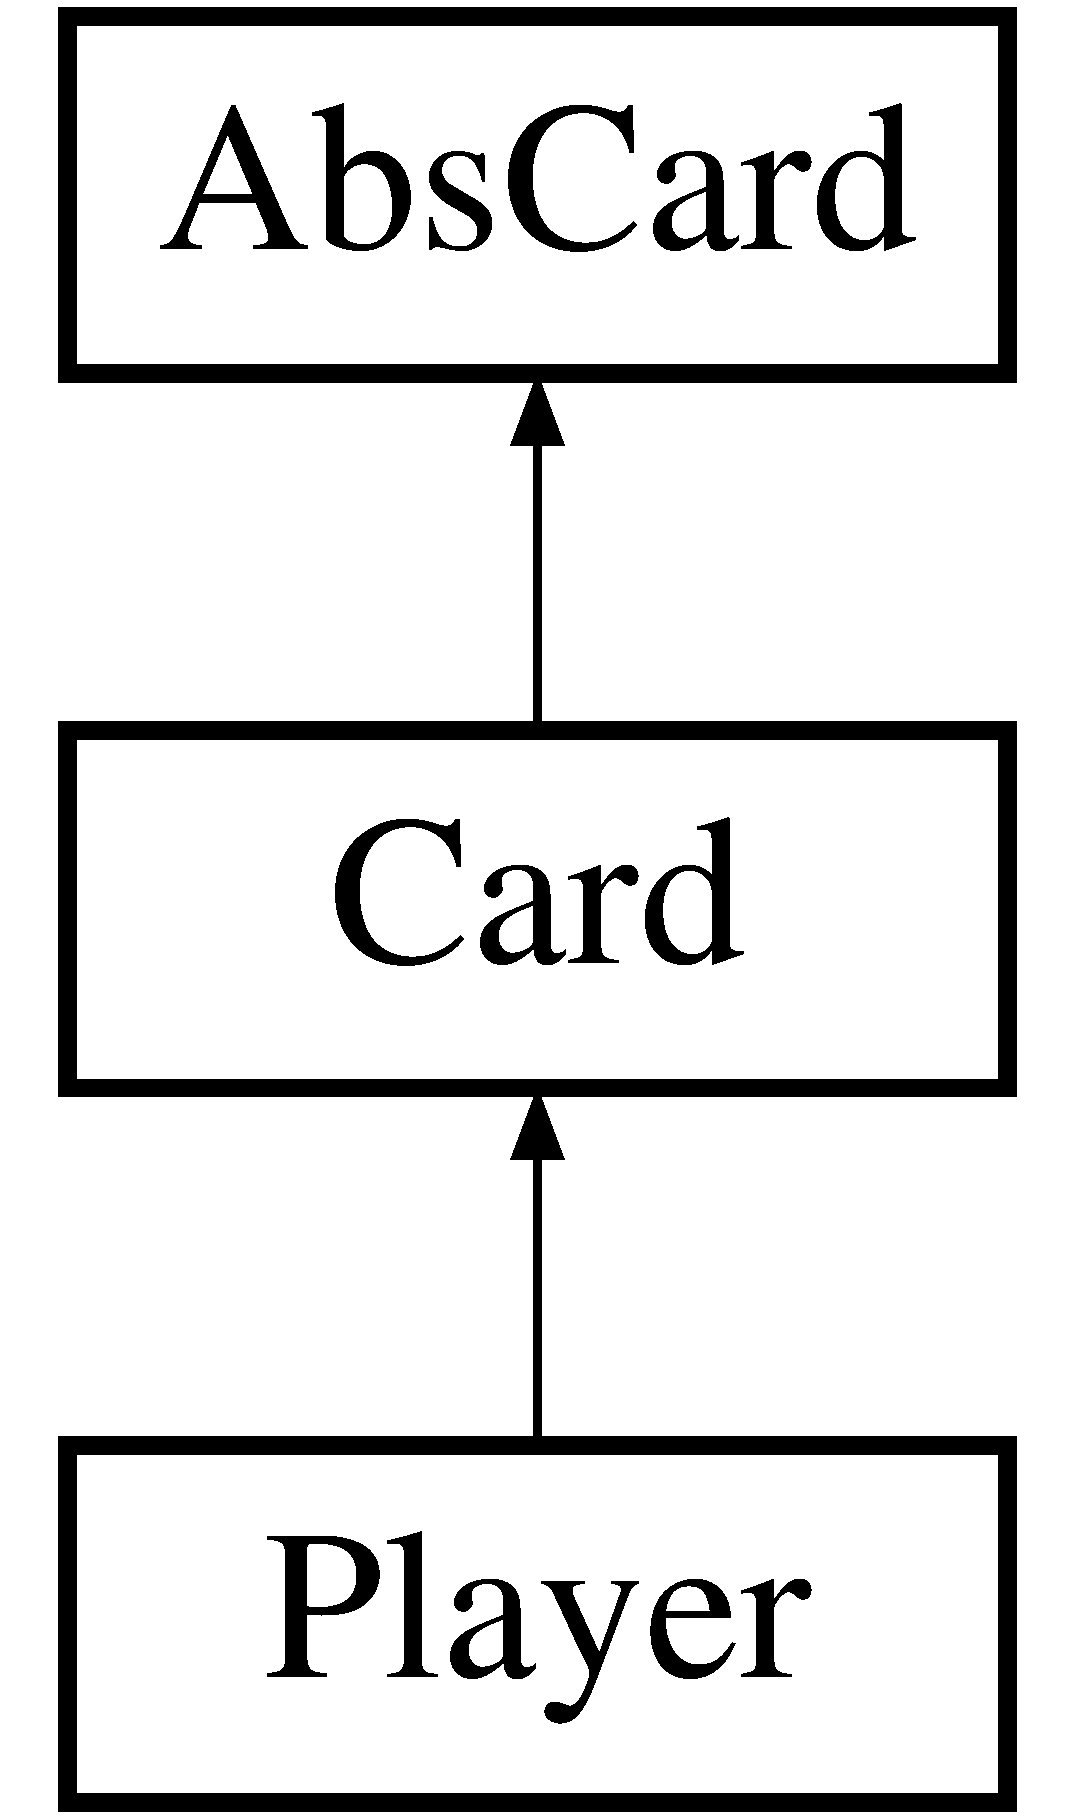
\includegraphics[height=3.000000cm]{class_abs_card}
\end{center}
\end{figure}
\subsection*{Private Member Functions}
\begin{DoxyCompactItemize}
\item 
\hypertarget{class_abs_card_a6238689463855fa406fb6aedf1e0aed4}{}\label{class_abs_card_a6238689463855fa406fb6aedf1e0aed4} 
virtual void {\bfseries set\+Num} (int)=0
\end{DoxyCompactItemize}


The documentation for this class was generated from the following file\+:\begin{DoxyCompactItemize}
\item 
/\+Users/siliguo/\+Desktop/\+Project\+\_\+2.\+5/Abs\+Card.\+h\end{DoxyCompactItemize}

\hypertarget{class_card}{}\section{Card Class Reference}
\label{class_card}\index{Card@{Card}}
Inheritance diagram for Card\+:\begin{figure}[H]
\begin{center}
\leavevmode
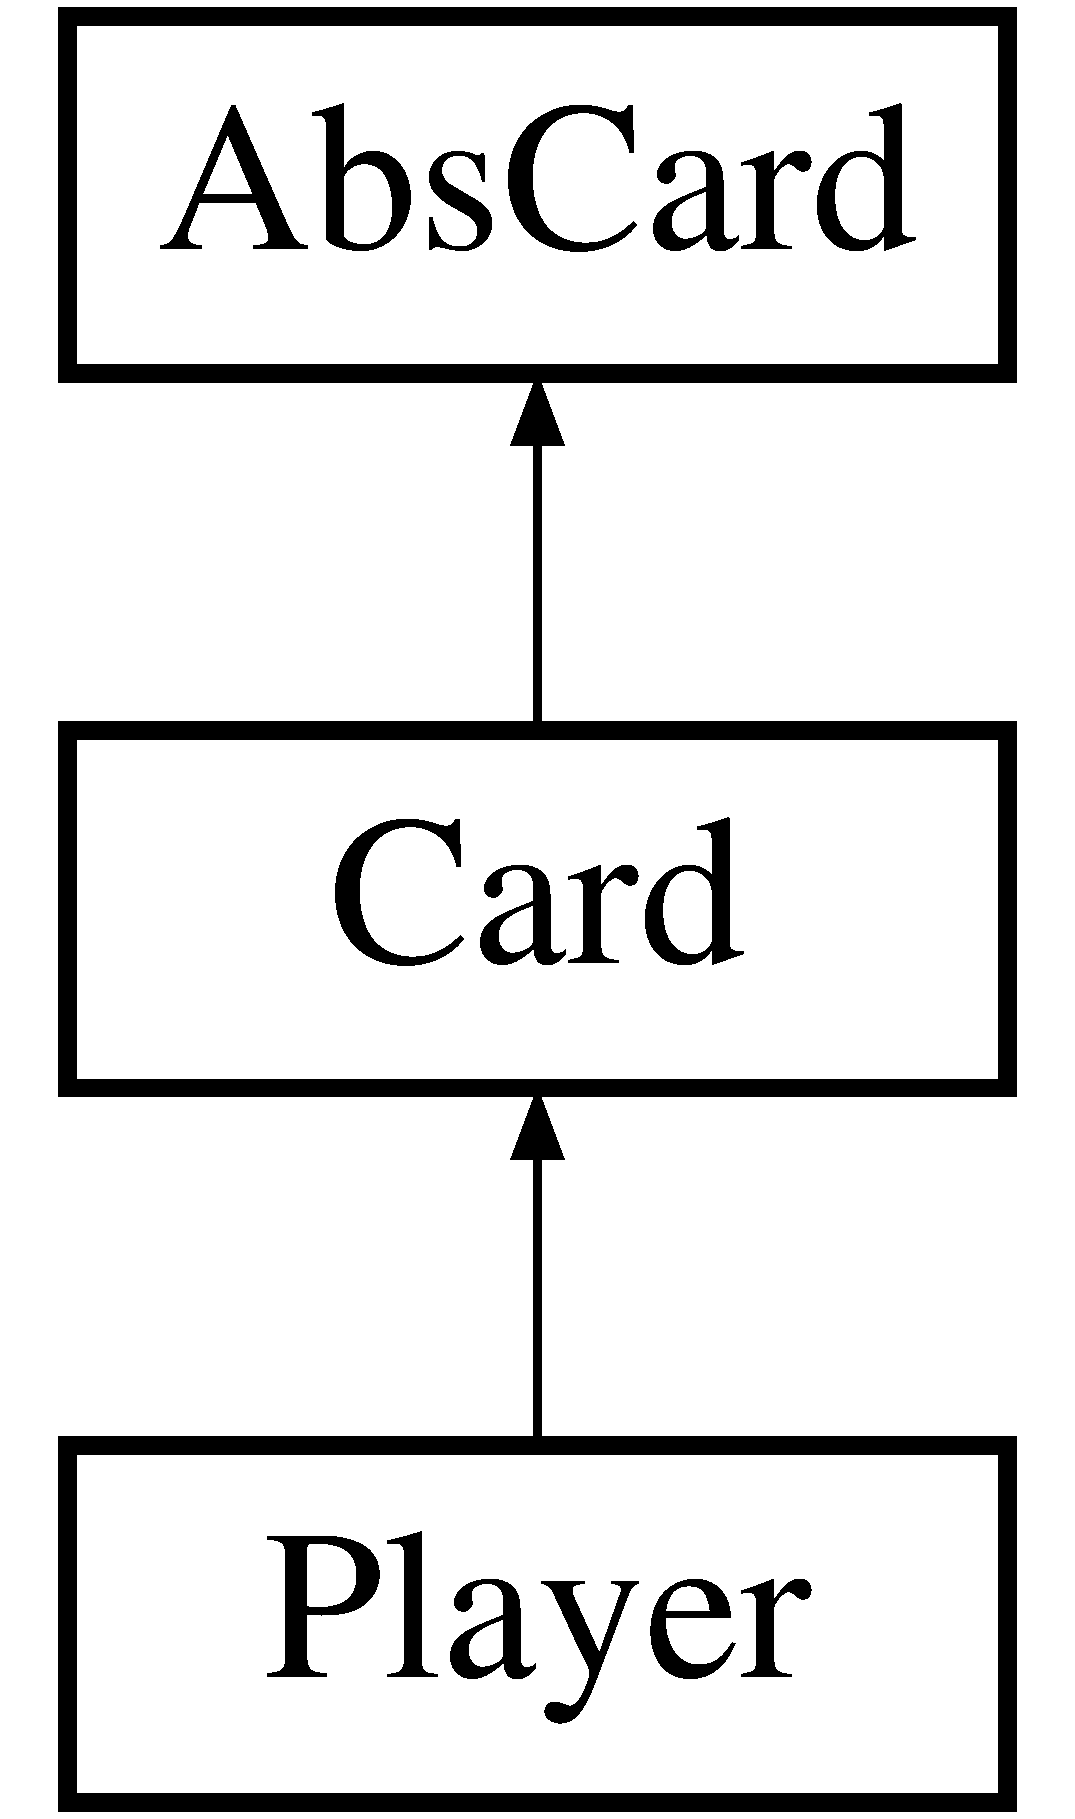
\includegraphics[height=3.000000cm]{class_card}
\end{center}
\end{figure}
\subsection*{Public Member Functions}
\begin{DoxyCompactItemize}
\item 
\hypertarget{class_card_ae45525322c984d687aef5fef969a7197}{}\label{class_card_ae45525322c984d687aef5fef969a7197} 
void {\bfseries set\+Num} (int)
\item 
\hypertarget{class_card_afdd26a7d861f1dae28dd967b3491fdd3}{}\label{class_card_afdd26a7d861f1dae28dd967b3491fdd3} 
int {\bfseries get\+Num} () const
\item 
\hypertarget{class_card_abfb09282f9920c235b464fb7f714b56c}{}\label{class_card_abfb09282f9920c235b464fb7f714b56c} 
char {\bfseries get\+Suit} ()
\item 
\hypertarget{class_card_a7b4e9a445eebedb4aa38cb9320a48207}{}\label{class_card_a7b4e9a445eebedb4aa38cb9320a48207} 
char {\bfseries get\+Name} ()
\item 
\hypertarget{class_card_a3df85ce283a6e38b719ffe25f3d4610a}{}\label{class_card_a3df85ce283a6e38b719ffe25f3d4610a} 
int {\bfseries get\+Value} ()
\end{DoxyCompactItemize}
\subsection*{Private Attributes}
\begin{DoxyCompactItemize}
\item 
\hypertarget{class_card_ad4ebd4bfe9458aeef44714093b4e2c5c}{}\label{class_card_ad4ebd4bfe9458aeef44714093b4e2c5c} 
int {\bfseries number}
\item 
\hypertarget{class_card_a164b95e624c7e21134ba535ddb28963b}{}\label{class_card_a164b95e624c7e21134ba535ddb28963b} 
char {\bfseries suit}
\item 
\hypertarget{class_card_af488f1f1bc0cfbbfe9a10676429ca1c1}{}\label{class_card_af488f1f1bc0cfbbfe9a10676429ca1c1} 
char {\bfseries name}
\item 
\hypertarget{class_card_a57c4269cef032dac1f282c9b2be3be4d}{}\label{class_card_a57c4269cef032dac1f282c9b2be3be4d} 
int {\bfseries value}
\end{DoxyCompactItemize}


The documentation for this class was generated from the following files\+:\begin{DoxyCompactItemize}
\item 
/\+Users/siliguo/\+Desktop/\+Project\+\_\+2.\+5/Card.\+h\item 
/\+Users/siliguo/\+Desktop/\+Project\+\_\+2.\+5/Card.\+cpp\end{DoxyCompactItemize}

\hypertarget{class_player}{}\section{Player Class Reference}
\label{class_player}\index{Player@{Player}}
Inheritance diagram for Player\+:\begin{figure}[H]
\begin{center}
\leavevmode
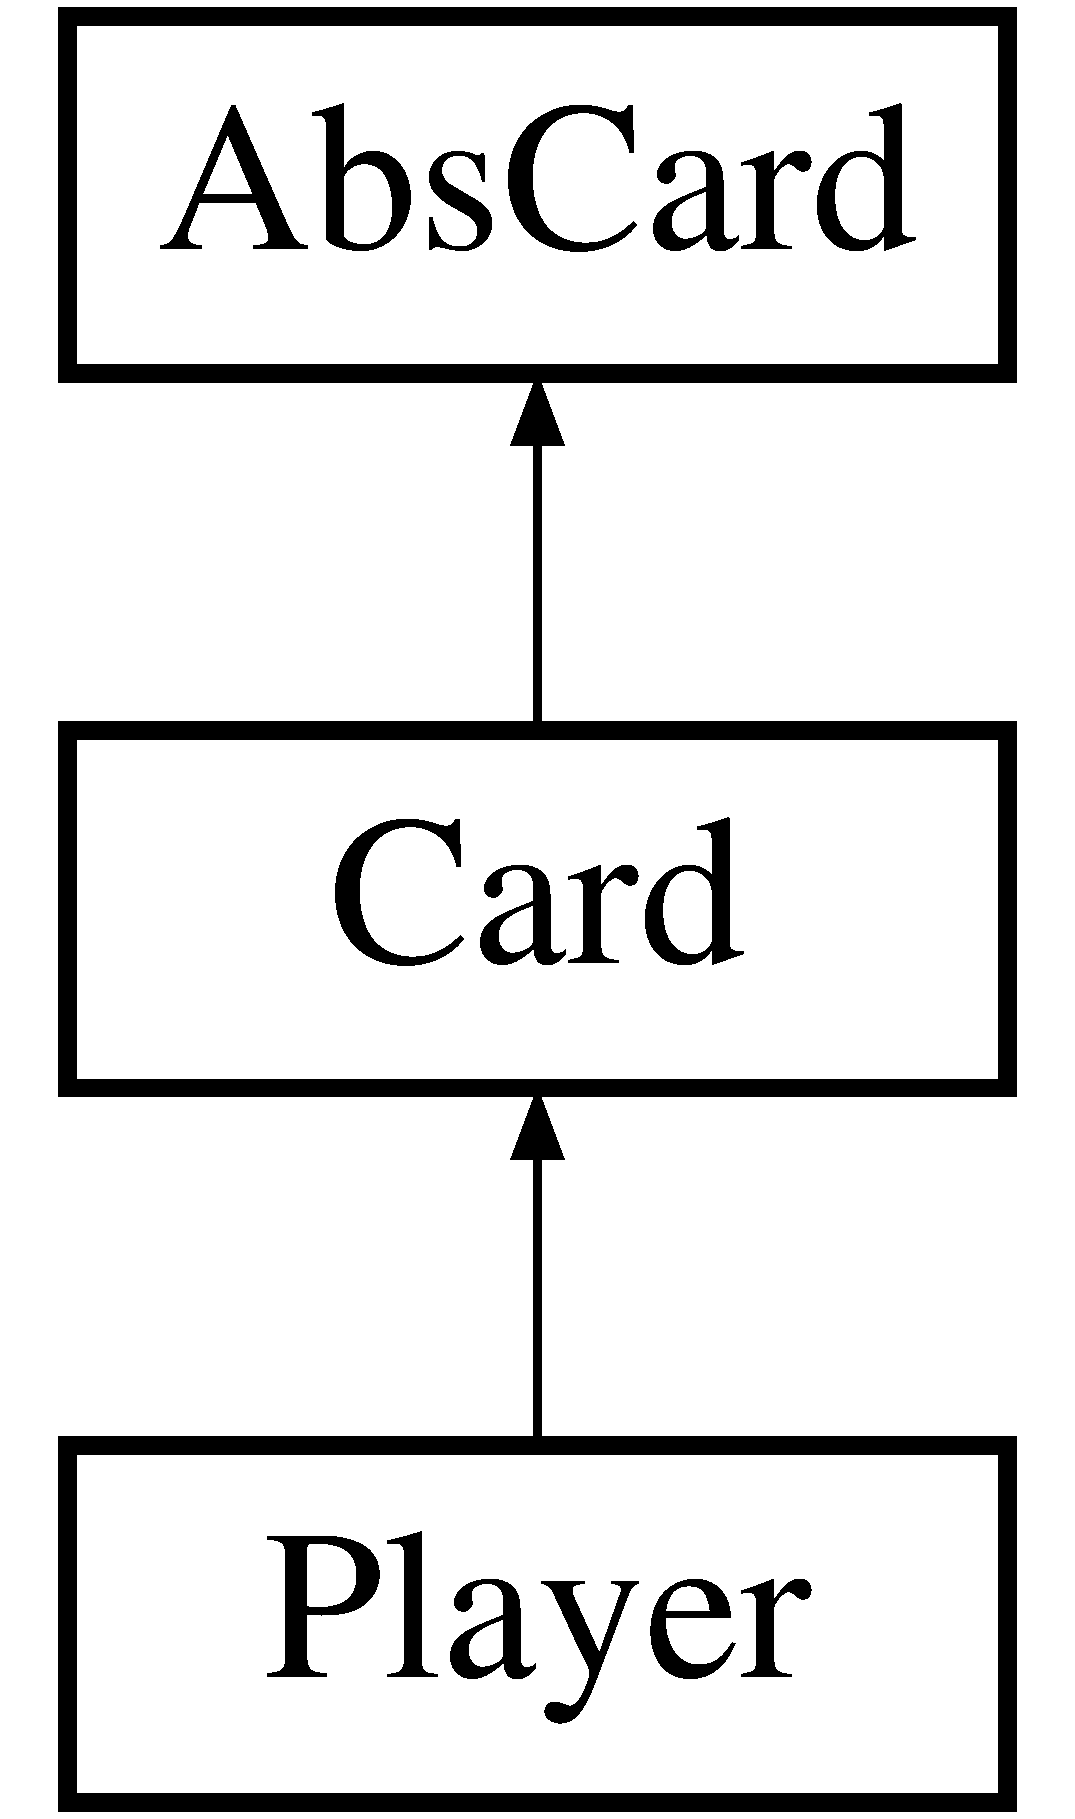
\includegraphics[height=3.000000cm]{class_player}
\end{center}
\end{figure}
\subsection*{Classes}
\begin{DoxyCompactItemize}
\item 
class \hyperlink{class_player_1_1_too_large}{Too\+Large}
\item 
class \hyperlink{class_player_1_1_too_small}{Too\+Small}
\end{DoxyCompactItemize}
\subsection*{Public Member Functions}
\begin{DoxyCompactItemize}
\item 
\hypertarget{class_player_a590858bfa3e172bee3c7c3a00168683a}{}\label{class_player_a590858bfa3e172bee3c7c3a00168683a} 
void {\bfseries set\+Card} (\hyperlink{struct_ply_num}{Ply\+Num})
\item 
\hypertarget{class_player_a384903af63898cdfb4e0bface7a65d6e}{}\label{class_player_a384903af63898cdfb4e0bface7a65d6e} 
void {\bfseries set\+Rank} ()
\item 
\hypertarget{class_player_aac509fade64f5bfbf6014ea3c2e3e5ea}{}\label{class_player_aac509fade64f5bfbf6014ea3c2e3e5ea} 
void {\bfseries set\+Money} (int m)
\item 
\hypertarget{class_player_a7a4239edef8f2ae2d88e4691819997d9}{}\label{class_player_a7a4239edef8f2ae2d88e4691819997d9} 
void {\bfseries set\+Bet} (int b)
\item 
\hypertarget{class_player_a6944db2ca2b4fd6736ef57be8b4abc05}{}\label{class_player_a6944db2ca2b4fd6736ef57be8b4abc05} 
\hyperlink{class_card}{Card} $\ast$ {\bfseries get\+Card} () const
\item 
\hypertarget{class_player_a903c68ffc821cba6e813a4d3b0b4c770}{}\label{class_player_a903c68ffc821cba6e813a4d3b0b4c770} 
int {\bfseries get\+Rank} () const
\item 
\hypertarget{class_player_aed6ceb1d2d434747fbea5a7fc9f829e4}{}\label{class_player_aed6ceb1d2d434747fbea5a7fc9f829e4} 
int {\bfseries get\+Money} () const
\item 
\hypertarget{class_player_af72bd8540101dd0f76c4a00c6b3a7982}{}\label{class_player_af72bd8540101dd0f76c4a00c6b3a7982} 
int {\bfseries get\+Bet} () const
\item 
\hypertarget{class_player_ada245979b1652b1d7795269cf73c1a6b}{}\label{class_player_ada245979b1652b1d7795269cf73c1a6b} 
bool {\bfseries operator$>$} (const \hyperlink{class_player}{Player} \&)
\end{DoxyCompactItemize}
\subsection*{Static Public Member Functions}
\begin{DoxyCompactItemize}
\item 
\hypertarget{class_player_ad60125d6e71ec216c68708e1460a2acb}{}\label{class_player_ad60125d6e71ec216c68708e1460a2acb} 
static void {\bfseries set\+Tbet} (int)
\item 
\hypertarget{class_player_ae04b689fe6a30486d457524fdee04643}{}\label{class_player_ae04b689fe6a30486d457524fdee04643} 
static int {\bfseries get\+Tbet} ()
\end{DoxyCompactItemize}
\subsection*{Private Attributes}
\begin{DoxyCompactItemize}
\item 
\hypertarget{class_player_a63492e432ef43e5f1e972fd75d1a28ee}{}\label{class_player_a63492e432ef43e5f1e972fd75d1a28ee} 
\hyperlink{class_card}{Card} $\ast$ {\bfseries card}
\item 
\hypertarget{class_player_a307c222c67b1318ec1d7dc9095c50a98}{}\label{class_player_a307c222c67b1318ec1d7dc9095c50a98} 
int {\bfseries rank}
\item 
\hypertarget{class_player_a9545beef70350d5c3b3a5719a890dd2f}{}\label{class_player_a9545beef70350d5c3b3a5719a890dd2f} 
int {\bfseries money}
\item 
\hypertarget{class_player_a9ad8e498594182ced9e8091de332f6d0}{}\label{class_player_a9ad8e498594182ced9e8091de332f6d0} 
int {\bfseries bet}
\end{DoxyCompactItemize}
\subsection*{Static Private Attributes}
\begin{DoxyCompactItemize}
\item 
\hypertarget{class_player_a0d3d76e3e84fffd06d0cd5af4def0260}{}\label{class_player_a0d3d76e3e84fffd06d0cd5af4def0260} 
static int {\bfseries Tbet} = 0
\end{DoxyCompactItemize}


The documentation for this class was generated from the following files\+:\begin{DoxyCompactItemize}
\item 
/\+Users/siliguo/\+Desktop/\+Project\+\_\+2.\+5/Player.\+h\item 
/\+Users/siliguo/\+Desktop/\+Project\+\_\+2.\+5/Player.\+cpp\end{DoxyCompactItemize}

\hypertarget{struct_ply_num}{}\section{Ply\+Num Struct Reference}
\label{struct_ply_num}\index{Ply\+Num@{Ply\+Num}}
\subsection*{Public Attributes}
\begin{DoxyCompactItemize}
\item 
\hypertarget{struct_ply_num_a25556b4ba727ee27041741546631a468}{}\label{struct_ply_num_a25556b4ba727ee27041741546631a468} 
int {\bfseries num} \mbox{[}3\mbox{]}
\end{DoxyCompactItemize}


The documentation for this struct was generated from the following file\+:\begin{DoxyCompactItemize}
\item 
/\+Users/siliguo/\+Desktop/\+Project\+\_\+2.\+5/Ply\+Num.\+h\end{DoxyCompactItemize}

\hypertarget{class_player_1_1_too_large}{}\section{Player\+:\+:Too\+Large Class Reference}
\label{class_player_1_1_too_large}\index{Player\+::\+Too\+Large@{Player\+::\+Too\+Large}}


The documentation for this class was generated from the following file\+:\begin{DoxyCompactItemize}
\item 
/\+Users/siliguo/\+Desktop/\+Project\+\_\+2.\+5/Player.\+h\end{DoxyCompactItemize}

\hypertarget{class_player_1_1_too_small}{}\section{Player\+:\+:Too\+Small Class Reference}
\label{class_player_1_1_too_small}\index{Player\+::\+Too\+Small@{Player\+::\+Too\+Small}}


The documentation for this class was generated from the following file\+:\begin{DoxyCompactItemize}
\item 
/\+Users/siliguo/\+Desktop/\+Project\+\_\+2.\+5/Player.\+h\end{DoxyCompactItemize}

%--- End generated contents ---

% Index
\backmatter
\newpage
\phantomsection
\clearemptydoublepage
\addcontentsline{toc}{chapter}{Index}
\printindex

\end{document}
